% !TEX root = main.tex
\section{Ativos e Passivos}

\begin{frame}[c]\frametitle{}

  \textbf{Ativos:} são bens e recursos que uma pessoa possui e que têm o potencial de gerar benefícios financeiros no futuro.
  \begin{itemize}
    \item Investimentos
    \item Imóveis
    \item Tudo aquilo que te gera renda.
  \end{itemize}
\end{frame}


\begin{frame}[c]\frametitle{}
  \textbf{Passivos:} são as obrigações financeiras que uma pessoa tem e que precisarão ser pagas no futuros, como:
  \begin{itemize}
    \item Compras no Cartão de Crédito.
    \item Empréstimos.
    \item Parcelamentos.
    \item Impostos.
    \item Tudo aquilo que te gera despesa.
  \end{itemize}
\end{frame}


\begin{frame}[c]\frametitle{O fluxo do dinhero}
  \begin{center}
    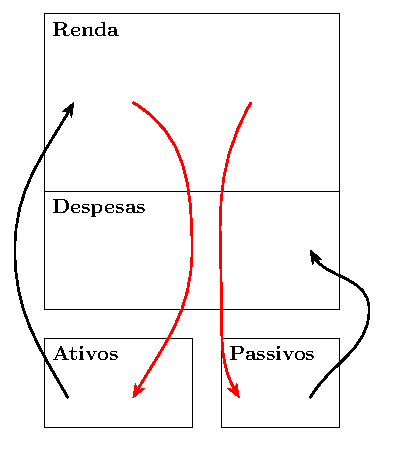
\includegraphics{../figuras/pai_rico}
  \end{center}
\end{frame}

\begin{frame}[c]
  \frametitle{}
  \begin{columns}
    \begin{column}{0.5\textwidth}
      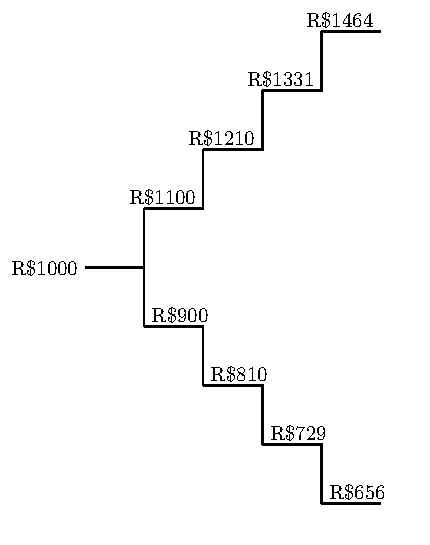
\includegraphics[width=\textwidth]{../figuras/dobra4.pdf}
    \end{column}
    \begin{column}{0.5\textwidth}
      \centering
      \textbf{\large Ao final de 4 anos um ativo rendendo de 10\% a.a. vale mais que o dobro de um passivo que desvaloriza na mesma taxa.}
      % \begin{itemize}
      %   \item Taxa de juros anual de 10\% a.a.
      %   \item $\frac{\text{R\$ 1464}}{\text{R\$656}} = 2,23$.
      %   \item Tentar gerar renda extra.
      %   \item Não aumentar os gastos devido a aumento salarial.
      % \end{itemize}
    \end{column}
  \end{columns}
\end{frame}